% \iffalse
% stb-beamer.dtx
% Copyright (C) 2023 Stellenbosch University
% All rights reserved.
%
% -------------------------------------------------------------------
% Stellenbosch University beamer presentation styles
% -------------------------------------------------------------------
%
% Author:     Danie Els
% Maintained: Danie Els (dnjels@sun.ac.za)
%
% This work may be distributed and modified, and must be credited
% under the conditions of the latest version of the Creative Commons 
% License (CC BY 4.0). The latest version of this license is in
% 
%    https://creativecommons.org/licenses/by/4.0/
% 
% -------------------------------------------------------------------
%
%<*driver>
\listfiles
\documentclass[a4paper]{ltxdoc}
\usepackage{stb-titlepage}
\usepackage{fourier}%.......................... Roman+math - Utopia
\usepackage{textcomp}%......................... Additional text symbols
\usepackage[scaled=0.85]{berasans}%............ Sans serif - Bera sans
\usepackage[scaled=0.85]{beramono}%............ Typewriter - Bera mono
\usepackage{xcolor}
    \definecolor{lstkey1}  {rgb} {0.65,0.04,0.07} % red
    \definecolor{lstkey0}  {rgb} {0.06,0.44,0.08} % green
    \definecolor{lstcomm}  {gray}{0.50}
    \definecolor{lstback}  {gray}{0.94}
    \definecolor{lstfrme}  {gray}{0.75}
\usepackage{stb-nomencl}
\usepackage{graphicx}
\makeatletter
%==== Additional documenting commands ==========================
\def\meta@font@select{\normalfont\ttfamily\itshape}
\newcommand*{\pkg}[1]{\textsf{#1}}
\newcommand*{\env}[1]{\texttt{#1}}
\newcommand*{\opt}[1]{\texttt{#1}}

%==== Define an environment for command/environment declarations.
\makeatletter
\usepackage{listings}
    \lstset{
        gobble=2,
        alsodigit={-0123456789_},
        columns=flexible,
        keepspaces,
        escapechar=|,
        basicstyle=\small\ttfamily,
        keywords=[0]{\title,\subtitle,\author,\institute,\date,\titlefig},
        keywordstyle=[0]\color{lstkey0},
        keywords=[1]{masters-a,masters-t,PhD,a5block,
                    goldenblock,wideblock,stdblock,stb-thesis},
        keywordstyle=[1]\color{lstkey1},
        comment=[l]\%,
        commentstyle=\color{lstcomm}\slshape,
        backgroundcolor=\color{lstback},
        belowskip=\medskipamount,
        aboveskip=\medskipamount,
        }
    \lstnewenvironment{ltxexample}[1][]{\lstset{#1}}{}


%\newsavebox{\declbox}
%\newenvironment{decl}{%
%  \begin{lrbox}{\declbox}
%     \small
%     \begin{tabular}{l}}
% {\end{tabular}\end{lrbox}%
%  \par\medskip\noindent\hspace*{2\parindent}\fbox{\usebox{\declbox}}\par\medskip}

\makeatother

\EnableCrossrefs
%\CodelineIndex
\CodelineNumbered
\RecordChanges
\setlength\hfuzz{15pt}
\hbadness=7000
\begin{document}
  \DocInput{stb-beamer.dtx}
\end{document}
%</driver>
% \fi
%
% \CheckSum{185}
%
% \CharacterTable
%  {Upper-case    \A\B\C\D\E\F\G\H\I\J\K\L\M\N\O\P\Q\R\S\T\U\V\W\X\Y\Z
%   Lower-case    \a\b\c\d\e\f\g\h\i\j\k\l\m\n\o\p\q\r\s\t\u\v\w\x\y\z
%   Digits        \0\1\2\3\4\5\6\7\8\9
%   Exclamation   \!     Double quote  \"     Hash (number) \#
%   Dollar        \$     Percent       \%     Ampersand     \&
%   Acute accent  \'     Left paren    \(     Right paren   \)
%   Asterisk      \*     Plus          \+     Comma         \,
%   Minus         \-     Point         \.     Solidus       \/
%   Colon         \:     Semicolon     \;     Less than     \<
%   Equals        \=     Greater than  \>     Question mark \?
%   Commercial at \@     Left bracket  \[     Backslash     \\
%   Right bracket \]     Circumflex    \^     Underscore    \_
%   Grave accent  \`     Left brace    \{     Vertical bar  \|
%   Right brace   \}     Tilde         \~}
%
% \changes{v1.0}{2023/07/26}{Initial version}
%
% ^^A== Title =====================================================
%
% \GetFileInfo{stb-beamer-a.sty}
% \title{The \textbf{\pkg{stb-beamer}} packages\thanks{^^A
%            This document corresponds to \pkg{stb-beamer}~v1.0, 
%            dated 2023/08/10.}}
% \author{Danie Els\\[1ex]
%         \normalsize e-mail: \texttt{dnjels@sun.ac.za}}
% \address{Department of Mechanical and Mechatronic Engineering\\
%         Stellenbosch University \\
%         Private Bag X1, Matieland 7602,\\ South Africa.}
% \date{2023/08/10}
%
% ^^A==============================================================
% \maketitle
% \begin{abstract}\centering
%    Presentation templates  Stellenbosch.
% \end{abstract}
% \sloppy
%
% \tableofcontents
% \clearpage
%
% ^^A==============================================================
% \section{Usage}
% \subsection{\pkg{stb-beamer-a}}
% \begin{ltxexample}
%   \documentclass[xcolor={svgnames,table},10pt,fleqn]{beamer}
%   \usepackage{stb-beamer-a}
%   
%   %---- Fonts ------------------------------------------------------------
%   \usefonttheme{professionalfonts}
%   \usepackage[T1]{fontenc}
%   \usepackage{textcomp}
%   \usepackage[default,medium,scaled=1.0]{raleway}
%   \usepackage[scaled=0.80]{arevmath}
%   
%   %---- Title page -------------------------------------------------------
%   \title[Ballistic\\ Gel]
%         {\Large DEM Modeling of Ballistic Gelatin for Low Energy Impacts}
%   %\subtitle{}
%   \author{\textbf{HC Grobbelaar\and DNJ Els\and CJ Coetzee}}
%   \institute{\itshape Dept of Mech \& Mechatronic Eng,\\
%              Stellenbosch University, South Africa}
%   \date{4th Aspherix and CFDEM Conference\\[0.5ex]
%         \small 20--21 Apr 2023, Linz, Austria}
%   \def\titlefig{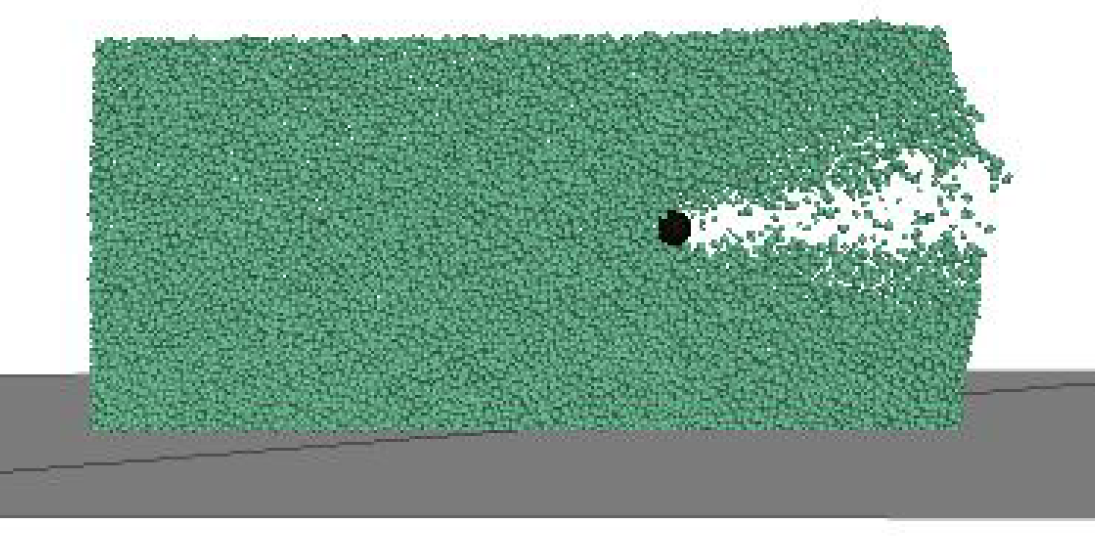
\includegraphics[width=7.0cm]{Ball-penetrate}}
% \end{ltxexample}
%
% \begin{figure}[htbp]
% \centering
% \fbox{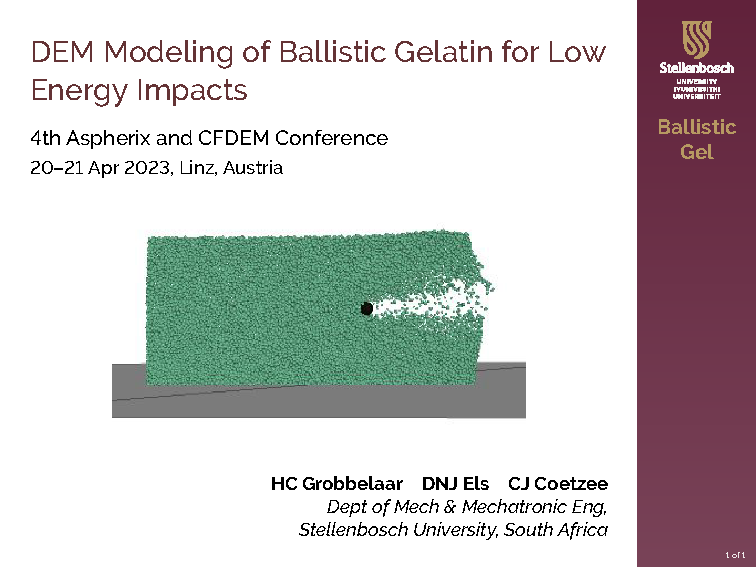
\includegraphics[width=0.85\hsize]{figs/stb-beamer-fig-a}}
% \caption{\pkg{stb-beamer-a}}
%\end{figure} 
% \clearpage
%
% \subsection{\pkg{stb-beamer-b}}
% \begin{ltxexample}
%   \documentclass[xcolor={svgnames,table},10pt,fleqn]{beamer}
%   \usepackage{stb-beamer-b}
%   
%   %---- Fonts ------------------------------------------------------------
%   \usefonttheme{professionalfonts}
%   \usepackage[T1]{fontenc}
%   \usepackage{textcomp}
%   \usepackage[default,medium,scaled=1.0]{raleway}
%   \usepackage[scaled=0.80]{arevmath}
%   
%   %---- Title page -------------------------------------------------------
%   \title[Ballistic\\ Gel]
%         {DEM Modeling of Ballistic Gelatin for Low Energy Impacts}
%   %\subtitle{}
%   \author[Grobbelaar et al]
%          {{\bfseries HC Grobbelaar\and DNJ Els\and CJ Coetzee}}
%   \institute[]{\itshape Dept of Mech \& Mechatronic Eng,\\
%              Stellenbosch University, South Africa}
%   \date[]{4th Aspherix and CFDEM Conference\\[0.5ex]
%         \small 20--21 Apr 2023, Linz, Austria}
%   \def\titlefig{}
% \end{ltxexample}
%
% \begin{figure}[htbp]
% \centering
% \fbox{
\includegraphics[width=0.85\hsize]{figs/stb-beamer-fig-b}}
% \caption{\pkg{stb-beamer-b}}
%\end{figure} 
%
% \clearpage
% \StopEventually{\PrintChanges\PrintIndex}
% ^^A==============================================================
%
% \section{Implementation: \pkg{stb-beamer}}
%    \subsection{Identification}
%
%    \begin{macrocode}
%<*beamer-a|beamer-b>
%    \end{macrocode}
%    \begin{macrocode}
\NeedsTeXFormat{LaTeX2e}
%    \end{macrocode}
%    \begin{macrocode}
%<*beamer-a>
\ProvidesPackage{stb-beamer-a}
                [2023/08/10 v1.0 Stellenbosch Beamer (DNJ ELS)]
%</beamer-a>
%    \end{macrocode}
%
%    \begin{macrocode}
%<*beamer-b>
\ProvidesPackage{stb-beamer-b}
                [2023/08/10 v1.0 Stellenbosch Beamer (DNJ ELS)]
%</beamer-b>
%    \end{macrocode}
%
%    \subsection{Colors}
%
%    \begin{macrocode}
\definecolor{stbMaroon}{RGB}{97,  34, 59}
\definecolor{stbGold}  {RGB}{183,153, 98}
\definecolor{stbGreen} {RGB}{130,204,174}
\definecolor{stbOrange}{RGB}{220, 68,  5}
\definecolor{stbWine}  {RGB}{166, 10, 61}
\definecolor{stbSoil}  {RGB}{100, 51, 53}
%    \end{macrocode}
%
%
%
% \subsection{\pkg{stb-beamer-a}}
%
%    \begin{macrocode}
%<*beamer-a>
\usetheme[]{Marburg}

\logo{
\includegraphics[width=1.25cm]{stb-logo-beamer}}

\useoutertheme[height=0pt,width=2cm,right]{sidebar}
\useinnertheme[shadow]{rounded}
\usecolortheme{rose,sidebartab}

\setbeamertemplate{sidebar canvas \beamer@sidebarside}
                  [vertical shading]
                  [top=stbMaroon,bottom=stbMaroon!85]

\setbeamertemplate{section in sidebar}{\vbox{%
    \beamer@sidebarformat{3pt}{section in sidebar}{\insertsectionhead}}}
\setbeamertemplate{section in sidebar shaded}{\vbox{%
    \beamer@sidebarformat{3pt}{section in sidebar shaded}{\insertsectionhead}}}

\setbeamertemplate{subsection in sidebar}{\vbox{%
    \beamer@sidebarformat{6pt}{subsection in sidebar}{\insertsubsectionhead}}}
\setbeamertemplate{subsection in sidebar shaded}{\vbox{%
        \beamer@sidebarformat{6pt}{subsection in sidebar shaded}{\insertsubsectionhead}}}

\usefonttheme[only large]{structurebold}

\setbeamercolor{structure}{fg=stbSoil}
\setbeamercolor{author}{parent=structure}
\setbeamercolor{title in sidebar}{fg=stbGold}

\setbeamerfont{title}{series=\normalfont,size=\Huge}
\setbeamerfont{title in sidebar}{series=\bfseries,size=\normalsize}
\setbeamerfont{author in sidebar}{series=\bfseries}
\setbeamerfont*{item}{series=}
\setbeamerfont{frametitle}{size=}
\setbeamerfont{block title}{size=\small}
\setbeamerfont{subtitle}{size=\Large,series=\normalfont}

\setbeamertemplate{navigation symbols}{}
\setbeamertemplate{bibliography item}[book]

\setbeamertemplate{sidebar right}
    {\hspace*{0pt}%
     \vskip2.5em%
     \hbox to2cm{\hss\insertlogo\hss}
    %\vskip1.25em%
    {\usebeamerfont{title in sidebar}%
     \vskip0.5em%
     \hskip3pt%
     \usebeamercolor[fg]{title in sidebar}%
     \insertshorttitle[width=\dimexpr 2cm-6pt,center,respectlinebreaks]\par%
     \vskip0.5em}%
     %\hbox to2cm{\hss\insertlogo\hss}
     %\vskip1.25em%
      \insertverticalnavigation{2cm}%
      \vfill
      \hbox to 2cm{\hfill
                   \usebeamerfont{subsection in sidebar}\strut
                   \usebeamercolor[fg]{subsection in sidebar}%
                   \insertframenumber{} of \inserttotalframenumber{}\hskip5pt}%
      \vskip3pt}%

\let\titlefig\relax
\setbeamertemplate{title page}
   {\vbox{}
    %\vskip1em
    {\usebeamercolor[fg]{title}\usebeamerfont{title}\inserttitle\par}%
    \ifx\insertsubtitle\@empty%
    \else%
        \vskip0.25em%
        {\usebeamerfont{subtitle}\usebeamercolor[fg]{subtitle}\insertsubtitle\par}%
    \fi%
    \vskip1em\par
    \insertdate\par
    \vskip0pt plus1filll
    \mbox{}\hfill\titlefig\hfill\mbox{}\par
    \vskip0pt plus1filll
    \leftskip=0pt plus1fill\insertauthor\par
    \insertinstitute\vskip1em}

\setbeamerfont{frametitle}{size=\large}
\setbeamercolor{frametitle}{bg=white,fg=stbMaroon}%{parent=block title}
\setbeamerfont{framesubtitle}{size=\normalsize, shape=\itshape}

\setbeamercolor{block title}{bg=stbMaroon!35,fg=stbMaroon}
\setbeamercolor{block body} {bg=stbMaroon!15,fg=black}

\setbeamercolor{block title alerted}{fg=white, bg=stbOrange}
\setbeamercolor{block body alerted}{bg=stbOrange!15,fg=stbOrange}
\setbeamercolor{alerted text}{fg=stbOrange}

\setbeamercolor{block title example}{fg=white, bg=stbGreen!70!black}
\setbeamercolor{block body example}{bg=stbGreen!25}
%</beamer-a>
%    \end{macrocode}
%
% \subsection{\pkg{stb-beamer-b}}
%
%    \begin{macrocode}
%<*beamer-b>
\usetheme[secheader]{Madrid}

\definecolor{stbGray}  {RGB}{140,151,154}  % 0.54, 0.59, 0.6
\definecolor{stbBlue}  {RGB}{  0, 99,150}

\setbeamercolor{titlelike}{bg=stbMaroon,fg=stbGold}
\setbeamercolor{palette primary}{bg=stbMaroon,fg=stbGold}
\setbeamercolor{palette secondary}{bg=stbMaroon,fg=stbGold}
\setbeamercolor{palette tertiary}{bg=stbMaroon,fg=stbGold}
\setbeamercolor{item projected}{fg=stbMaroon, bg=stbMaroon}

\setbeamercolor{block title}{bg=stbMaroon,fg=stbGold}
\setbeamercolor{block body}{bg=stbGray!35,fg=black}

\setbeamercolor{block title alerted}{fg=white, bg=stbOrange}
\setbeamercolor{block body alerted}{bg=stbOrange!15,fg=stbOrange}
\setbeamercolor{alerted text}{fg=stbOrange}

\setbeamercolor{block title example}{fg=white, bg=stbGreen!70!black}
\setbeamercolor{block body example}{bg=stbGreen!25}


\setbeamerfont{block body}{size=\small}
\setbeamerfont{block body example}{size=\small}
\setbeamerfont{block body alerted}{size=\small}

\setbeamerfont{frametitle}{size=\normalsize}
\setbeamerfont{block title}{size=\normalsize}
\setbeamerfont{block title example}{size=\normalsize}

\setbeamertemplate{title}{%
    \begin{beamercolorbox}[sep=2pt,left]{title}
    \raisebox{-0.575\height}{
\includegraphics[width=3cm]{stb-logo-horiz-w}}
    \hfill
    \parbox[t]{\dimexpr\hsize-3cm-4pt-8pt}{%
            \usebeamerfont{title}\inserttitle%
            \ifx\insertsubtitle\@empty%
            \else%
              \par\vskip0.25em%
              {\usebeamerfont{subtitle}\usebeamercolor[fg]{subtitle}\insertsubtitle}%
            \fi}%    
    \end{beamercolorbox}%
}
%</beamer-b>
%    \end{macrocode}
%
%    \begin{macrocode}
%</beamer-a|beamer-b>
%    \end{macrocode}
%
%    The end of this package.
%    \Finale
\endinput


